
%(BEGIN_QUESTION)
% Copyright 2014, Tony R. Kuphaldt, released under the Creative Commons Attribution License (v 1.0)
% This means you may do almost anything with this work of mine, so long as you give me proper credit

The following power and trip circuit diagrams show the differential current (87) protection for a large three-phase generator:

$$\includegraphics[width=15.5cm]{i03070x01.eps}$$

Suppose one day the 86 relay trips, opening all three circuit breakers (52-P, 52-N, and 41) and illuminating the ``Tripped'' lamp.  Electricians subsequently perform continuity and high-voltage insulation tests of the stator windings within the generator but find no faults at all.

\vskip 10pt

Identify the likelihood of each specified fault for this system.  Consider each fault one at a time (i.e. no coincidental faults), determining whether or not each fault could independently account for {\it all} measurements and symptoms in this circuit.

% No blank lines allowed between lines of an \halign structure!
% I use comments (%) instead, so that TeX doesn't choke.

$$\vbox{\offinterlineskip
\halign{\strut
\vrule \quad\hfil # \ \hfil & 
\vrule \quad\hfil # \ \hfil & 
\vrule \quad\hfil # \ \hfil \vrule \cr
\noalign{\hrule}
%
% First row
{\bf Fault} & {\bf Possible} & {\bf Impossible} \cr
%
\noalign{\hrule}
%
% Another row
Dead DC station power supply &  &  \cr
%
\noalign{\hrule}
%
% Another row
Fault in generator field winding &  &  \cr
%
\noalign{\hrule}
%
% Another row
CT failed open &  &  \cr
%
\noalign{\hrule}
%
% Another row
86 trip coil failed open &  &  \cr
%
\noalign{\hrule}
%
% Another row
86 trip coil failed shorted &  &  \cr
%
\noalign{\hrule}
%
% Another row
Any 87/SI coil failed open &  &  \cr
%
\noalign{\hrule}
%
% Another row
Any 87/SI coil failed shorted &  &  \cr
%
\noalign{\hrule}
%
% Another row
Any 87/RC coil failed open &  &  \cr
%
\noalign{\hrule}
%
% Another row
Any 87/RC coil failed shorted &  &  \cr
%
\noalign{\hrule}
%
% Another row
Any 87/OC coil failed open &  &  \cr
%
\noalign{\hrule}
%
% Another row
Any 87/OC coil failed shorted &  &  \cr
%
\noalign{\hrule}
} % End of \halign 
}$$ % End of \vbox


\underbar{file i03070}
%(END_QUESTION)





%(BEGIN_ANSWER)

\noindent
{\bf Partial answer:}

% No blank lines allowed between lines of an \halign structure!
% I use comments (%) instead, so that TeX doesn't choke.

$$\vbox{\offinterlineskip
\halign{\strut
\vrule \quad\hfil # \ \hfil & 
\vrule \quad\hfil # \ \hfil & 
\vrule \quad\hfil # \ \hfil \vrule \cr
\noalign{\hrule}
%
% First row
{\bf Fault} & {\bf Possible} & {\bf Impossible} \cr
%
\noalign{\hrule}
%
% Another row
Dead DC station power supply &  &  \cr
%
\noalign{\hrule}
%
% Another row
Fault in generator field winding &  &  \cr
%
\noalign{\hrule}
%
% Another row
CT failed open &  &  \cr
%
\noalign{\hrule}
%
% Another row
86 trip coil failed open &  & $\surd$ \cr
%
\noalign{\hrule}
%
% Another row
86 trip coil failed shorted &  &  \cr
%
\noalign{\hrule}
%
% Another row
Any 87/SI coil failed open &  &  \cr
%
\noalign{\hrule}
%
% Another row
Any 87/SI coil failed shorted &  &  \cr
%
\noalign{\hrule}
%
% Another row
Any 87/RC coil failed open & $\surd$ &  \cr
%
\noalign{\hrule}
%
% Another row
Any 87/RC coil failed shorted &  &  \cr
%
\noalign{\hrule}
%
% Another row
Any 87/OC coil failed open &  &  \cr
%
\noalign{\hrule}
%
% Another row
Any 87/OC coil failed shorted &  &  \cr
%
\noalign{\hrule}
} % End of \halign 
}$$ % End of \vbox
 
%(END_ANSWER)





%(BEGIN_NOTES)

% No blank lines allowed between lines of an \halign structure!
% I use comments (%) instead, so that TeX doesn't choke.

$$\vbox{\offinterlineskip
\halign{\strut
\vrule \quad\hfil # \ \hfil & 
\vrule \quad\hfil # \ \hfil & 
\vrule \quad\hfil # \ \hfil \vrule \cr
\noalign{\hrule}
%
% First row
{\bf Fault} & {\bf Possible} & {\bf Impossible} \cr
%
\noalign{\hrule}
%
% Another row
Dead DC station power supply &  & $\surd$ \cr
%
\noalign{\hrule}
%
% Another row
Fault in generator field winding &  & $\surd$ \cr
%
\noalign{\hrule}
%
% Another row
CT failed open & $\surd$ &  \cr
%
\noalign{\hrule}
%
% Another row
86 trip coil failed open &  & $\surd$ \cr
%
\noalign{\hrule}
%
% Another row
86 trip coil failed shorted &  & $\surd$ \cr
%
\noalign{\hrule}
%
% Another row
87/SI coil failed open &  & $\surd$ \cr
%
\noalign{\hrule}
%
% Another row
87/SI coil failed shorted &  & $\surd$ \cr
%
\noalign{\hrule}
%
% Another row
87/RC coil failed open & $\surd$ &  \cr
%
\noalign{\hrule}
%
% Another row
87/RC coil failed shorted & $\surd$ &  \cr
%
\noalign{\hrule}
%
% Another row
87/OC coil failed open &  & $\surd$ \cr
%
\noalign{\hrule}
%
% Another row
87/OC coil failed shorted &  & $\surd$ \cr
%
\noalign{\hrule}
} % End of \halign 
}$$ % End of \vbox

%INDEX% Electric power systems: protective relays (differential)
%INDEX% Electronics review: current transformer (CT)
%INDEX% Protective relay: differential current (87)
%INDEX% Protective relay: troubleshooting

%(END_NOTES)


